\chapter{Results}
\label{ch:results}

Everything in this chapter was measured on the system itself. No person other
than the author has used it, and no result here involves a physical arm moving
under load. Where a quantity has never been measured, the text says so.

\section{When the instrument is the fault}
\label{sec:instruments}

This section comes first because it changes how the rest should be read.

Seventeen times in six weeks, a result that looked like a fault in the robot
turned out to be a fault in the thing measuring the robot. Not seventeen small
discrepancies: seventeen occasions on which a confident, specific and wrong
number was produced and would have been believed.

\begin{table}[htbp]
  \centering
  \small
  \caption[Instrument faults]{A selection of the measurement faults found in
  this project, with the mechanism in each. The pattern is the useful part:
  none of them announced itself, and every one produced a plausible number.}
  \label{tab:instruments}
  \begin{tabular}{@{}p{0.40\linewidth}p{0.54\linewidth}@{}}
    \toprule
    \textbf{What was reported} & \textbf{What was actually happening} \\
    \midrule
    Sensor noise of exactly zero on all fourteen channels & The recorder
      writes rows three times faster than the sensors update, so most rows are
      copies of the one before \\
    Object detection succeeding on 0--4\,\% of frames & The synthetic test
      images were flat coloured rectangles; the same detector scores 0.89 on a
      photograph \\
    A measure of symmetry reading exactly zero & Sixteen failed lookups in a
      row. Perfect symmetry and an empty loop produce the same number \\
    A scene rendering correctly at 18\,\% ink coverage & The scene was empty.
      The wearer alone is 18\,\% of the frame \\
    Every waypoint of a task unreachable & The check was solving for the wrist
      pointing where the arm rests, not where the task actually sends it,
      \SI{43}{\degree} away \\
    A clearance of \SI{367}{\milli\metre} & The arm was physically touching the
      mannequin. The check samples the centres of joints and misses the arm
      between them, and it returns the same number for a clear pose \\
    An arm reported as stalled \SI{360}{\degree} from its target & Three of the
      joints turn continuously, so $-179$ and $+181$ degrees are the same
      position. The move had finished \\
    A test suite reporting a failing test called \texttt{=} & The style checker
      echoes the lines it objects to, and one source file contained the word
      FAILED inside a string \\
    \bottomrule
  \end{tabular}
\end{table}

The working rule that came out of this is short. A surprising result is
evidence about the instrument until the instrument has been cleared. In
practice that means every analysis program is given an input whose answer is
already known and has to return it; a check that cannot be made to fail on a
deliberately broken input is not a check; and a result that contradicts an
earlier measurement is treated as an instrument problem until the two are
reconciled.

The last of those is easy to skip and is the one that pays. Two figures for
the same quantity, produced by different programs on different days, disagreed
by a factor of five. The instinct is to trust the newer one. Reconciling them
found that the older program had been asking a different question for weeks.

\section{The master arm}

Six of fourteen channels currently meet the health criterion, and the
distribution of failures is not random: five of the six failures are on one
arm, which points at wiring rather than at the sensors.

Replaying recorded traces with the driver's hand held still, and with only the
failing channels allowed to move, gives the size of the problem. On the worse
arm the failing channels alone command \SI{54.5}{\milli\metre} of hand
movement, against a master reach of \SI{272}{\milli\metre}. On the better arm
the equivalent figure is \SI{0.014}{\milli\metre}. There is no filter that
rescues the first number, because the values are not noisy: they are wrong and
they are steady.

The processing chain itself contributes nothing. Feeding it a constant input
produces a constant output to within the deadband, which is the control
result that lets the \SI{54.5}{\milli\metre} be attributed to the sensors
rather than to the software reading them.

\section{Where the commands go}

Vertical and forward-and-back commands map correctly on both arms. Sideways
does not, and the reason is geometric rather than a matter of which sign
convention was used.

\begin{figure}[htbp]
  \centering
  % Two movements the driver makes at right angles arrive 137.7 degrees apart.
\begin{tikzpicture}[x=1mm, y=1mm, font=\scriptsize]

  % intended
  \begin{scope}[shift={(0,0)}]
    \node[font=\small\bfseries, anchor=south] at (18,26) {What the driver did};
    \draw[go, thick] (0,0) -- (24,0) node[right, font=\scriptsize] {sideways};
    \draw[go, thick] (0,0) -- (0,22) node[above, font=\scriptsize] {forward};
    \draw[gray] (5,0) arc (0:90:5);
    \node[font=\scriptsize] at (9,7) {\SI{90}{\degree}};
  \end{scope}

  % measured
  \begin{scope}[shift={(62,0)}]
    \node[font=\small\bfseries, anchor=south] at (18,26) {Where the arm was sent};
    \draw[go, thick, red!65!black] (0,0) -- (24,0)
      node[right, font=\scriptsize] {first movement};
    \draw[go, thick, red!65!black] (0,0) -- (-16.3,14.8)
      node[above left, font=\scriptsize, align=center] {second\\ movement};
    \draw[gray] (6,0) arc (0:137.7:6);
    \node[font=\scriptsize, red!65!black] at (7,11) {\SI{137.7}{\degree}};
  \end{scope}

  \node[tag, text width=112mm, align=left] at (40,-14)
    {Two directions that ought to be at right angles arrive
     \SI{47.7}{\degree} apart from where they should be. This is a property of
     the geometry, not of the labelling: three directions that are not
     mutually perpendicular cannot be made perpendicular by swapping or
     negating axes, and no setting in the software can do it. Fixing it means
     moving a sensor or adding one.};

\end{tikzpicture}

  \caption[The sideways problem]{Two movements the driver makes at right
  angles to each other arrive \SI{137.7}{\degree} apart at the robot. The test
  is deliberately independent of any axis labelling, which is what makes this
  a geometric limit rather than a calibration error.}
  \label{fig:lateral}
\end{figure}

The mechanism is that sideways movement is estimated from a single shoulder
sensor whose axis is not aligned with the direction the driver perceives as
sideways. Fixing it needs either the sensor moved or a second one added; it
does not need software.

\section{The workspace}

This section contains the project's main negative result.

\begin{figure}[htbp]
  \centering
  
\includegraphics[width=0.95\linewidth]{reach_directions.pdf}
  \caption[How far the arms reach, by direction]{Reach from the resting pose
  in the six principal directions, with the wearer in the model, as the median
  of ten sweeps. The label inside each bar is what stopped the arm. In sixteen
  of the twenty-six directions measured, that is either a collision or the
  arm's inability to fold into the shape required, and almost never the length
  of the arm. \emph{Max range} means the sweep ran out of travel before the
  arm did, so those figures are lower bounds.}
  \label{fig:reach}
\end{figure}

\begin{figure}[htbp]
  \centering
  
\includegraphics[width=0.86\linewidth]{workspace_disjoint.pdf}
  \caption[The two arms do not meet]{Points in front of the wearer that each
  arm can reach. The two sets do not overlap anywhere, and there is a gap of
  about a quarter of a metre between them straddling the body's centre line.
  Measured over a grid of sixty-three positions with the wearer present; with
  the wearer removed entirely, three shared points appear, and the wearer
  removes all three.}
  \label{fig:disjoint}
\end{figure}

Four separate measurements were made because the first result was surprising
enough to distrust. Sweeping the height of the working surface and the
distance to it, over 3\,360 combinations, with the objects resting on the
surface rather than floating above it, produced no arrangement at all in which
an object within \SI{100}{\milli\metre} of the wearer's centre line could be
picked up. With the wearer's own arms deleted from the model, the innermost
workable column moves in by \SI{25}{\milli\metre} on one side and
\SI{75}{\milli\metre} on the other, and the limit is then the torso. Asked for
a top-down grasp instead of an approach from the side, the answer is zero
positions out of eight hundred and forty, at any surface height.

That is worth restating plainly, because it is the single most consequential
thing measured in this project. \textbf{The centre of a person's own working
space is the one place a pair of shoulder-mounted arms cannot go}, and no
change to the control software affects it.

\begin{figure}[htbp]
  \centering
  
\includegraphics[width=0.86\linewidth]{mount_sweep.pdf}
  \caption[What a mount change would buy]{Shared reachable positions against
  each mounting parameter, taken one at a time from the arrangement as built.
  Moving the mounts inboard and tilting them further forward both help, and
  they help together. Splaying them outward was measured separately and makes
  matters worse, which is why it does not appear here. The best buildable
  combination raises the shared count from three to twenty-two of sixty-three.}
  \label{fig:mount}
\end{figure}

\begin{figure}[htbp]
  \centering
  
\includegraphics[width=0.86\linewidth]{lateral_constraint.pdf}
  \caption[One boundary, two reasons]{Two independent constraints meet at
  roughly the same place. As the working area is moved outboard, clearance to
  the wearer rises through the floor at about \SI{0.25}{\metre}, and grasping
  from above becomes possible at about the same distance. The coincidence is
  not causal, and it means an object placed to satisfy one constraint tends to
  satisfy the other.}
  \label{fig:lateral-boundary}
\end{figure}

The mount change is quantified and has not been applied. Applying it
invalidates the resting pose, the approach direction written into every task,
and every clearance figure derived from either, so it is a deliberate
re-measurement of the whole system rather than an adjustment.

\begin{figure}[htbp]
  \centering
  
\includegraphics[width=0.95\linewidth]{clearance_tasks.pdf}
  \caption[Clearance during each task]{Closest approach to the wearer over the
  whole of each task's path, ten repeats, with the body measured
  geometrically. The grey label above each bar is the part of the body that
  was nearest. Only the pick-and-place task stays clear on both arms.
  \SI{161}{\milli\metre} appears three times because that is the mounting
  bracket, which no joint moves, so it is the best any pose can do. The
  breaches are reported rather than quietly fixed: moving a task's coordinates
  means re-verifying the whole task.}
  \label{fig:clearance}
\end{figure}

\section{Grasping, and why one task cannot be done}

The gripper opens \SI{85}{\milli\metre}. Measured from the positions of the
two finger pads, and taking the width each object presents along the closing
direction:

\begin{table}[htbp]
  \centering
  \small
  \caption[What fits in the hand]{The width each object presents to the
  gripper, along the direction the fingers close. The gripper opens
  \SI{85}{\milli\metre}.}
  \label{tab:grip}
  \begin{tabular}{@{}p{0.34\linewidth}rrl@{}}
    \toprule
    \textbf{Object} & \textbf{Side approach} & \textbf{From above} &
    \textbf{Fits?} \\
    \midrule
    \SI{40}{\milli\metre} block & \SI{49.0}{\milli\metre} &
      \SI{40.0}{\milli\metre} & yes, both ways \\
    Carry tray, left grip & \SI{83.4}{\milli\metre} & no solution & by
      \SI{1.6}{\milli\metre} \\
    Carry tray, right grip & \SI{113.9}{\milli\metre} & no solution &
      \textbf{no} \\
    Circuit box & \SI{195.0}{\milli\metre} & \SI{170.0}{\milli\metre} &
      \textbf{no, either way} \\
    Multimeter & \SI{42.4}{\milli\metre} & \SI{30.0}{\milli\metre} & yes \\
    \bottomrule
  \end{tabular}
\end{table}

Two of the four tasks are blocked by this table alone, and neither is a
control problem. They need a different object or a different gripper.

\section{Where the hand actually ends up}

For a grasp to close on an object the gripper has to arrive within about
\SI{30}{\milli\metre} of it. \Cref{fig:budget} is every known contribution to
missing that, measured separately.

\begin{figure}[htbp]
  \centering
  % THE POSITIONING ERROR BUDGET.
% Each term is measured separately by scripts/measure_control_budget.py and
% the pair of bars per row is the value before and after the correction that
% was applied, so the figure shows what the corrections bought rather than
% only the state they left behind. The unmeasured term is drawn as an open
% bar with no length, because giving it one would be an invention.
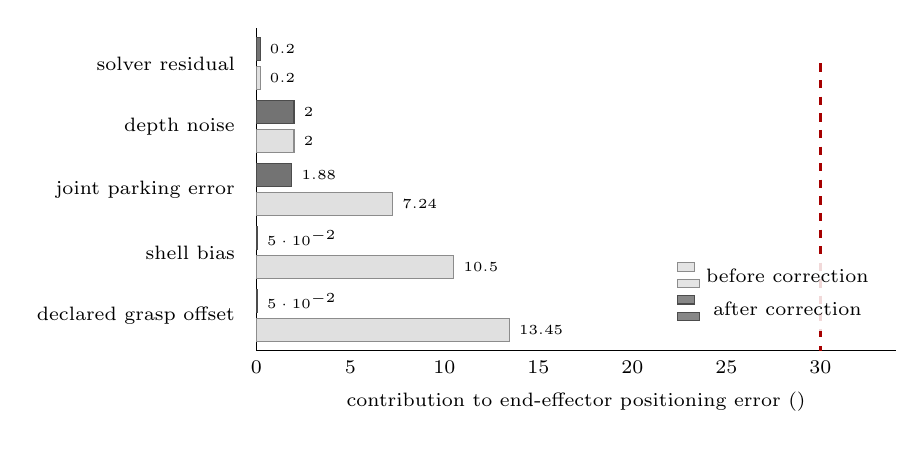
\begin{tikzpicture}
\begin{axis}[
    width=0.80\linewidth, height=64mm,
    xbar, y=8mm, bar width=3mm,
    xmin=0, xmax=34,
    xlabel={contribution to end-effector positioning error (\si{\milli\metre})},
    symbolic y coords={
      {camera mounting},
      {declared grasp offset},
      {shell bias},
      {joint parking error},
      {depth noise},
      {solver residual}},
    ytick=data,
    y tick label style={font=\scriptsize},
    x tick label style={font=\scriptsize},
    xlabel style={font=\scriptsize},
    nodes near coords, nodes near coords style={font=\tiny},
    every node near coord/.append style={anchor=west},
    enlarge y limits=0.14,
    axis lines*=left,
    tick style={draw=none},
    legend style={font=\scriptsize, at={(0.98,0.06)}, anchor=south east,
                  draw=none, fill=white, fill opacity=0.85,
                  text opacity=1, row sep=1pt},
]
\addplot[fill=black!12, draw=black!45] coordinates {
  (0.2,{solver residual})
  (2.0,{depth noise})
  (7.24,{joint parking error})
  (10.5,{shell bias})
  (13.45,{declared grasp offset})
};
\addlegendentry{before correction}
\addplot[fill=black!55, draw=black!70] coordinates {
  (0.2,{solver residual})
  (2.0,{depth noise})
  (1.88,{joint parking error})
  (0.05,{shell bias})
  (0.05,{declared grasp offset})
};
\addlegendentry{after correction}

% The unmeasured term. An open bar of no length, so it cannot be read as a
% quantity: there is no computer-aided design of the gripper module in this
% repository and the transform has never been measured.
\draw[black!55, dashed, thick] (axis cs:0,{camera mounting})
  rectangle (axis cs:9,{camera mounting});
\node[font=\tiny\itshape, anchor=west, black!55]
  at (axis cs:9.6,{camera mounting}) {not measured: the largest remaining unknown};

\draw[red!65!black, thick, dashed]
  (axis cs:30,{solver residual}) -- (axis cs:30,{camera mounting});
\node[font=\tiny, red!65!black, anchor=south east, align=right]
  at (axis cs:29.4,{camera mounting}) {\SI{30}{\milli\metre} capture gate};
\end{axis}
\end{tikzpicture}

  \caption[The error budget]{Contributions to positioning error at the moment
  of grasping. Grey bars are measured. The orange bar is the mounting of the
  camera relative to the arm, which has never been measured and is now the
  largest unknown. Adding the measured terms in the worst case gives
  \SI{33.4}{\milli\metre} against a \SI{30}{\milli\metre} requirement; combined
  in quadrature they give \SI{18.6}{\milli\metre}.}
  \label{fig:budget}
\end{figure}

Two of the three largest terms already have corrections written and switched
off, and with both enabled the worst case falls to about
\SI{17}{\milli\metre}. Both are switched off for the same reason: neither has
been tried on a physical arm, and enabling an untested correction would change
every recorded figure at once.

The unmeasured term is the one to go and measure. The camera's position is
computed from the model of the arm, which is exact given the model, and nobody
has ever checked the model against the physical camera module. A first attempt
at this on hardware suggests the error is angular rather than a simple offset:
the table cannot move, yet the direction of the table surface measured from
four different arm positions varied by \SI{8.45}{\degree}, which is
\SI{34}{\milli\metre} of position error at typical working distance. No
open-loop grasp planned through that can land inside the gate, and none did.

\section{The safety layer}

All fourteen injected faults are handled. The two timing figures worth
quoting: a master that has frozen but is still publishing is caught in
\SIrange{0.94}{0.99}{\second}, and the emergency stop now parks the arms
immediately rather than four seconds later.

\section{How fast the wearer would have to move}

This is the least comfortable result in the thesis and it is not a bug.

The clearance floor is a distance. The guard's knowledge of where the wearer
is arrives with a delay of between \SI{62}{\milli\second} and
\SI{562}{\milli\second}, the spread being a rate limit rather than the
tracking itself. Multiplying that delay by plausible limb speeds gives how far
a limb travels before the guard hears about it.

\begin{table}[htbp]
  \centering
  \small
  \caption[The reaction budget]{How far a limb moves before the guard knows,
  against a \SI{150}{\milli\metre} floor. Limb speeds are taken from the
  literature and are labelled as assumptions, not measurements.}
  \label{tab:reaction}
  \begin{tabular}{@{}llrl@{}}
    \toprule
    \textbf{Movement} & \textbf{Delay} & \textbf{Travel} & \textbf{Against the floor} \\
    \midrule
    A deliberate reach & \SI{62}{\milli\second} & \SIrange{50}{93}{\milli\metre} & 62\,\% of it \\
    A deliberate reach & \SI{562}{\milli\second} & \SIrange{450}{843}{\milli\metre} & exceeds it \\
    A quick reach & \SI{62}{\milli\second} & \SIrange{93}{155}{\milli\metre} & exceeds it \\
    A quick reach & \SI{562}{\milli\second} & \SIrange{843}{1405}{\milli\metre} & exceeds it \\
    A flinch & \SI{62}{\milli\second} & \SIrange{155}{248}{\milli\metre} & exceeds it \\
    A flinch & \SI{562}{\milli\second} & \SIrange{1405}{2248}{\milli\metre} & exceeds it \\
    \bottomrule
  \end{tabular}
\end{table}

In five of the six cases the limb travels further than the entire margin
before the system knows anything has changed. The floor is a distance, not a
reaction time, and nothing in this system currently reacts to a person moving
quickly. \Cref{ch:discussion} sets out the three things that would help and
what each would cost.

\section{Verification}

None of the figures above would be worth quoting without something behind them
that fails when the system changes. \Cref{tab:verification} is what that
amounts to at the date of writing. The two counts worth singling out are the
257 checks made on the operating window, which press every control and then
check what the press did, and the fourteen injected faults, because those two
are the only checks in the list that exercise the system the way a person
would.

\begin{table}[htbp]
  \centering
  \small
  \caption[Verification totals]{What is checked automatically, as of the date
  of writing.}
  \label{tab:verification}
  \begin{tabular}{@{}p{0.56\linewidth}r@{}}
    \toprule
    \textbf{Measure} & \textbf{Count} \\
    \midrule
    Automated tests passing & 1\,322 \\
    Test files & 114 \\
    Checks made on the operating window & 257 \\
    Faults injected and handled & 14 of 14 \\
    Recorded task demonstrations & 17 cells, 8 camera angles each \\
    Grasp success in those recordings & 100\,\% \\
    Analysis and verification programs & 233 \\
    Stored measurement records & 195 \\
    \bottomrule
  \end{tabular}
\end{table}

\section{What has not been measured}

The list is short and every item is a consequence of the same thing, which is
that no experiment has been run on a moving physical arm carrying a load.

Detection accuracy at working distance on the real cameras. The delay from the
driver's hand moving to the arm moving, end to end. The behaviour of the
control session when the arm's power is interrupted. Whether the sideways
mapping problem persists once the master is rewired. How the joint error
varies with speed, which was reported as measured and was not: the three
speeds turned out to be three repetitions of one condition, because the speed
limit was read once when the program started. And speech recognition against a
real speaker, which cannot be measured on this machine at all, because it has
no audio input device. Every voice figure in this project came from
synthesised speech and is a measure of the grammar rather than of the
recogniser.
